\section{Parceive}
\label{sec:parceive}
The goal of Parceive is to help developers in identifying parallelism
opportunities and obstacles at various granularity levels. It utilizes static
binary analysis and dynamic instrumentation to collect trace data. Being less
conservative than purely static approaches lets us consider a wider range of
possible scenarios. During execution, our tool focuses on concurrency-related
runtime events, e.g., memory accesses, routine invocations, and object
instantiations. By a-posteriori abstraction of such fine-grained information,
we infer architectural aspects from the applications. The results can be used
as a starting point for architecture redesign and refactoring. However, due to
the inherent incompleteness of dynamic analysis, the user is responsible for
correct parallelization.

\begin{figure}[h!]
	\begin{center}
		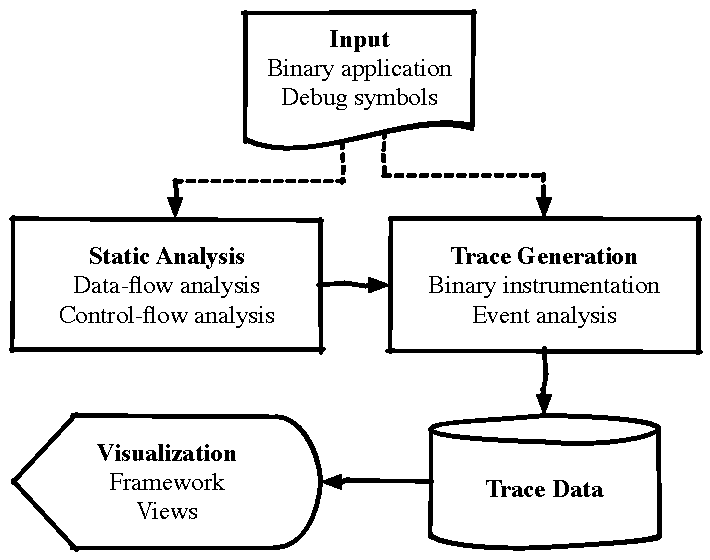
\includegraphics[width=0.40\textwidth]{img/parceive}
		\caption{The high-level components of Parceive.}
		\label{fig:parceive_overview}
	\end{center}
\end{figure}

Figure \ref{fig:parceive_overview} depicts the fundamental components of
Parceive and their relations. Our analyses operate on executables to retrieve
the required information. These analyses can be classified as static or dynamic
ones. The former inspect the data- and control-flow of single linkage objects.
By incorporating debug symbols, static analysis enables our tool to gather
information about variable accesses, loop constructs, and class hierarchies.
Additionally, the gathered information is used to restrict the scope of
subsequent runtime analysis in order to reduce the execution overhead.

Parceive instruments and inspects user applications on predefined events, e.g.,
object instantiations, method invocations, and thread handling (in case of
multi-threaded applications). During these events, the tool collects trace data
and stores it in an SQL database. The database scheme enables highly specific
and performant queries for different visualizations which are key for program
comprehension and parallelization. Each visualization thereby simplifies and
highlights specific aspects of the traced software.